\documentclass[11pt, a4paper]{article}
\usepackage{amsmath, amsthm, amssymb, calrsfs, wasysym, verbatim, bbm, color, graphics, geometry}
\usepackage[utf8]{inputenc} % comment when using lualatex
\usepackage[italian]{babel} % lingua e a-capo-sillabato
\usepackage{fullpage}
\usepackage{graphicx}
%\usepackage[hidelinks]{hyperref,xcolor} % link di pagina
\usepackage[bottom]{footmisc} % note appiccicate al fondo della pagina
\usepackage{float} % per posizionamento immagini
\usepackage{cancel}

\geometry{tmargin=.75in, bmargin=.75in, lmargin=.75in, rmargin = .75in}  

\newcommand{\R}{\mathbb{R}}
\newcommand{\C}{\mathbb{C}}
\newcommand{\Z}{\mathbb{Z}}
\newcommand{\N}{\mathbb{N}}
\newcommand{\Q}{\mathbb{Q}}
\newcommand{\Cdot}{\boldsymbol{\cdot}}

\newtheorem{thm}{Theorem}
\newtheorem{defn}{Definition}
\newtheorem{conv}{Convention}
\newtheorem{rem}{Remark}
\newtheorem{lem}{Lemma}
\newtheorem{cor}{Corollary}



\definecolor{dkgreen}{rgb}{0,0.6,0}
\definecolor{gray}{rgb}{0.5,0.5,0.5}
\definecolor{mauve}{rgb}{0.58,0,0.82}


\title{Distributed Systems}
\author{Raffaele Castagna}

\date{Academic Year 2025-2026}

\begin{document}

\maketitle

\tableofcontents
\newpage

\section{Introduction}
\begin{defn}
    In a system we have \textit{n} processes in $\prod:{p_{0}\dots,p_{n-1}}$ each with a distinct identity
    they communicate by utilizing a communication graph \textbf{G : ($\prod,E$)}, the communication is done by exchanging messages.

\end{defn}
\begin{center}
    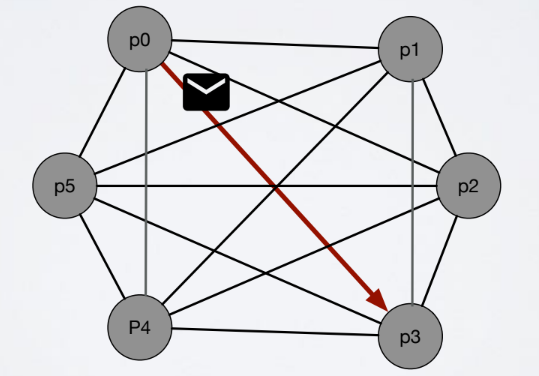
\includegraphics[scale=0.6]{img/comm graph}
\end{center}
\begin{defn}
A process is a (possibily infinite) State Machine (I/O Automaton).
\end{defn}
\begin{center}
    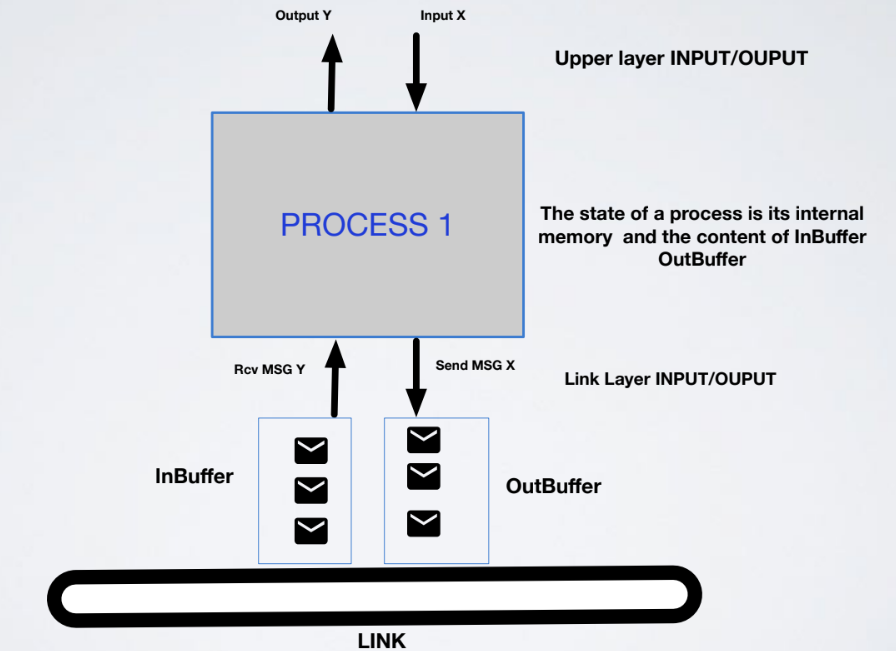
\includegraphics[scale=0.55]{img/process.png}
\end{center}
Each process has multiple qualities:
\begin{itemize}
    \item A set of internal states \textit{Q}
    \item A set of initial states $Q_i \subset Q$
    \item A set of all possible messages M in the form <sender,receiver,payload>
    \item Multiset of delivered messages $InBuf_j$
    \item Multiset of inflight messages $OutBuf_j$
\end{itemize}
\newpage
We can formally describe this as follows: (this isnt part of the exam btw) 
$$P_j (q \in Q \cup Q_{in},InBuf_j) = (q' \in Q, SendMsg \subset M \newline)$$  $$ OutBuf_j = OutBuf_j \cup SendMsg$$ $$\newline InBuf_j = \cancel{0}$$
To execute a process we have an adversary that schedules a set of events (scheduler), these events may be for example a delivery (e.g. Del(m,i,j)) or it can be one step of the step machine of process i (Exec(i))
\begin{defn}
    A configuration $C_t$ is a vector of n components, component j indicates the state of process j.
\end{defn}
\begin{center}
    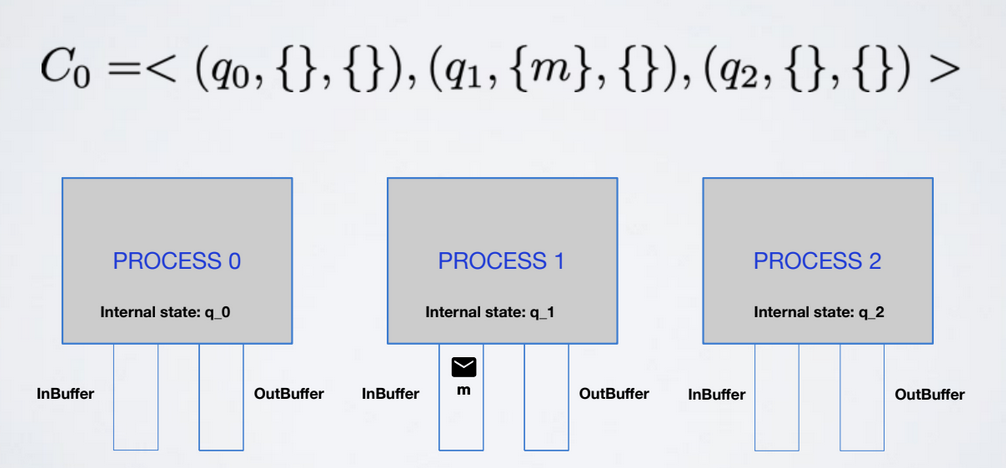
\includegraphics[scale=0.55]{img/configuration.png}
\end{center}
An event is \textbf{enabled} in configuration c if it can happen.
\begin{defn}
    An execution is an infinite sequence that alternates configurations and events: $(C_0,e_0,C_1,e_1,C_2,e_2,\dots)$ such that each event $e_t$ is enabled in configuration $C_t$ and $C_t$ is obtained by applying $e_{t-1} \text{ to } C_{t-1}$

\end{defn}
It may be useful to visualize how an execution involving multiple processes works, here we have an example:
\begin{center}
    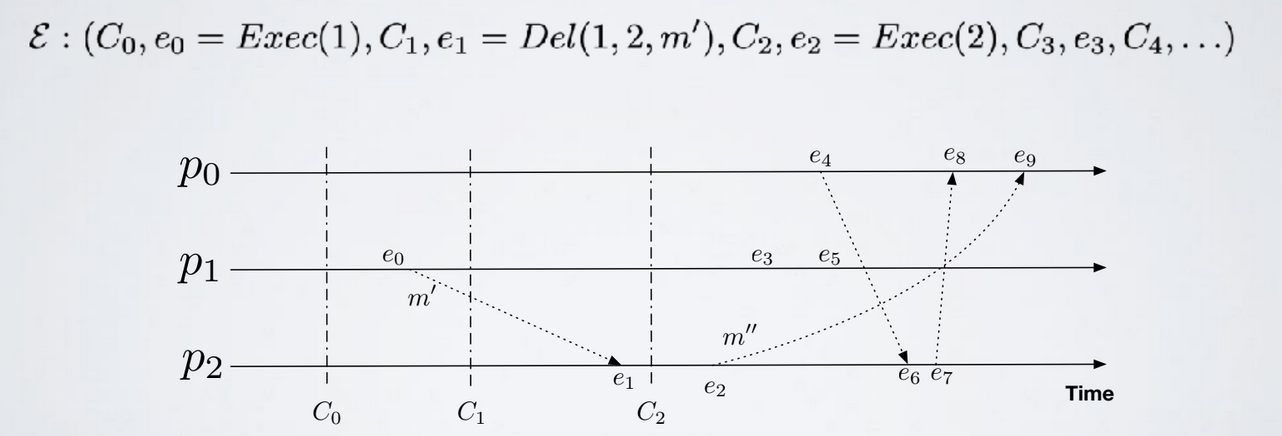
\includegraphics[scale=0.5]{img/execgraph.png}
\end{center}
\newpage
\begin{defn}
    A \textbf{fair execution} is an execution E where each process $p_i$ executes an infinite number of local computations (Exec(i) events are not finite) and each message m is eventually delivered (we can't stall messages)
\end{defn}
We will always use fair executions unless stated otherwise.
\begin{defn}
    Given an execution E and a procces $p_j$, we define the local view/ local execution of $E|p_j$ the subset of events in E that impact $p_j$
    \begin{center}
        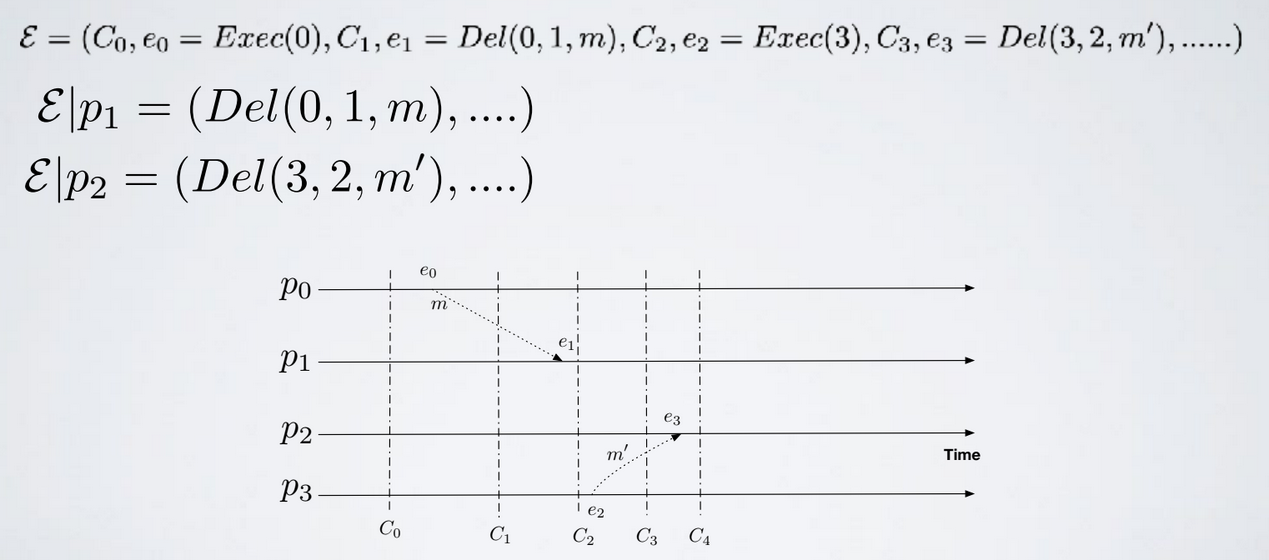
\includegraphics[scale=0.5]{img/localexec.png}
    \end{center}
\end{defn}
But these executions do not account for time, so we may have executions that are the same even though the events happened at different times, in case this does happen, we say that two executions are \textbf{\textit{indistinguishable}}.
\begin{thm}
In the asynch. model there is no distributed algorithm capable of reconstructing the system execution.
\end{thm}

\subsection{section}{Synchronous Vs Asynchronous}
We have 3 main types of synchrony:
\begin{itemize}
    \item Asynchronous Systems
    \item Eventually Synchronous Systems
    \item Synchronous systems
\end{itemize}
We can say that is a system is synchronous if it has a fixed bound on the daly of messages, on the time of actions executed by processes, and a fixed bound between execution of actions.
\subsection{Failures}
\end{document}